\documentclass[11pt]{report}
\usepackage[margin=2cm]{geometry}
\usepackage[dvipsnames]{xcolor}
\usepackage{graphicx}
\usepackage{float}
\usepackage{times}
\usepackage[numbers,sort&compress]{natbib}

\newcommand{\carbon}{\texorpdfstring{CO\textsubscript{2}}{CO2}}

\PassOptionsToPackage{hyphens}{url}\usepackage{hyperref}
\usepackage{fnpct}

\newcommand{\Gap}{\texorpdfstring{\hfill}{}}
\newcommand{\Rec}{\texorpdfstring{{\small\emph{\color{blue}{\fbox{High Leverage}}}}}{}}
\newcommand{\HighRisk}{\texorpdfstring{{\small\emph{\color{orange}{\fbox{Uncertain Impact}}}}}{}}
\newcommand{\Longterm}{\texorpdfstring{{\small\emph{\color{OliveGreen}{\fbox{Long-term}}}}}{}}

\setcounter{secnumdepth}{3}

\usepackage{color}
\newcommand{\maybe}[1]{{\color{red} #1}}

\begin{document}


\section{Electricity Systems\texorpdfstring{\hfill\textit{by Priya L.~Donti}}{}}
\label{sec:electricity-systems}
AI has been called the new electricity, given its potential to transform entire industries \cite{youtube2017andrew}. Interestingly, electricity itself is one of the industries that AI is poised to transform. Many electricity systems are awash in data, and the industry has begun to envision next-generation systems (\emph{smart grids}) driven by AI and ML \cite{ramchurn2012putting, perera2014machine, victor2019how}.

Electricity systems\footnote{Throughout this section, we use the term ``electricity systems'' to refer to the procurement of fuels and raw materials for electric grid components; the generation and storage of electricity; and the delivery of electricity to end-use consumers. For primers on these topics, see \cite{ipcc2014energy,federal2015energy, von2006electric, kirschen2004fundamentals, wood2013power}.} are responsible for about a quarter of human-caused greenhouse gas emissions each year \cite{ipcc2014summary}. Moreover, as buildings, transportation, and other sectors seek to replace GHG-emitting fuels (\S\ref{sec:transportation}-\ref{sec:buildings-cities}), demand for low-carbon electricity will grow. To reduce emissions from electricity systems, society must
\begin{itemize}
    \item Rapidly transition to low-carbon\footnote{We use the term ``low-carbon'' here instead of ``renewable'' because of this paper's explicit focus on climate change goals. Renewable energy is produced from inexhaustible or easily replenished energy sources such as the sun, wind, or water, but need not necessarily be carbon-free (as in the case of some biomass \cite{creutzig2016economic}). Similarly, not all low-carbon energy is renewable (as in the case of nuclear energy).} electricity sources (such as solar, wind, hydro, and nuclear) and phase out carbon-emitting sources (such as coal, natural gas, and other fossil fuels).
    \item Reduce emissions from existing \carbon-emitting power plants, since the transition to low-carbon power will not happen overnight.
    \item Implement these changes across all countries and contexts, as electricity systems are everywhere.
\end{itemize}

ML can contribute on all fronts by informing the research, deployment, and operation of electricity system technologies (Fig.~\ref{fig:electricitySystems}). Such contributions include accelerating the development of clean energy technologies, improving forecasts of demand and clean energy, improving electricity system optimization and management, and enhancing system monitoring. These contributions require a variety of ML paradigms and techniques, as well as close collaborations with the electricity industry and other experts to integrate insights from operations research, electrical engineering, physics, chemistry, the social sciences, and other fields.


\subsection{Enabling low-carbon electricity}
\label{sec:electricity-lowCarbon}
Low-carbon electricity sources are essential to tackling climate change. These sources come in two forms:~variable and controllable. Variable sources fluctuate based on external factors;~for instance, solar panels produce power only when the sun is shining, and wind turbines only when the wind is blowing. On the other hand, controllable sources such as nuclear or geothermal plants can be turned on and off (though not instantaneously\footnote{Nuclear power plants are often viewed as inflexible since they can take hours or days to turn on or off, and are often left on (at full capacity) to operate as \emph{baseload}. That said, nuclear power plants may have some flexibility to change their power generation for load-following and other electric grid services, as in the case of France \cite{lokhov2011technical}.}). These two types of sources affect electricity systems differently, and so present distinct opportunities for ML techniques.

\subsubsection{Variable sources}
\label{sec:electricity-variable}
Most electricity is delivered to consumers using a physical network called the electric grid, where the power generated must equal the power consumed at every moment. This implies that for every solar panel, wind turbine, or other variable electricity generator, there is some mix of natural gas plants, storage, or other controllable sources ready to buffer changes in its output (e.g.~when unexpected clouds block the sun or the wind blows less strongly than predicted). Today, this buffer is often provided by coal and natural gas plants run in a CO$_2$-emitting standby mode called \emph{spinning reserve}. In the future, this role is expected to be played by energy storage technologies such as batteries (\S\ref{sec:transport-evs}), pumped hydro, or power-to-gas~\cite{evans2012assessment}\footnote{It is worth noting that in systems with many fossil fuel plants, storage may increase emissions depending on how it is operated \cite{hittinger2015bulk, babacan2018unintended}.}.
ML can both reduce emissions from today's standby generators and enable the transition to carbon-free systems by helping improve necessary technologies (namely forecasting, scheduling, and control) and by helping create advanced electricity markets that accommodate both variable electricity and flexible demand.

\begin{figure}
    \centering
    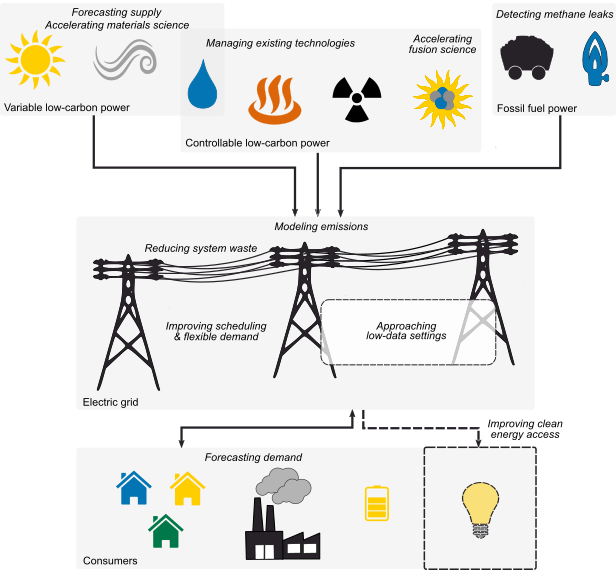
\includegraphics[width=.99\textwidth]{figures/electricity_systems.png}
    \caption{Selected opportunities to reduce GHG emissions from electricity systems using machine learning.}
    \label{fig:electricitySystems}
\end{figure}

\paragraph{Forecasting supply and demand}\Gap\textbf{\Rec}\mbox{}\\
Since variable generation and electricity demand both fluctuate, they must be forecast ahead of time to inform real-time electricity scheduling and longer-term system planning. Better short-term forecasts can allow system operators to reduce their reliance on polluting standby plants and to proactively manage increasing amounts of variable sources. Better long-term forecasts can help system operators (and investors) determine where and when variable plants should be built. While many system operators today use basic forecasting techniques, forecasts will need to become increasingly accurate, span multiple horizons in time and space, and better quantify uncertainty to support these use cases. ML can help on all these fronts.

To date, many ML methods have been used to forecast electricity supply and demand. These methods have employed historical data, physical model outputs, images, and even video data to create short- to medium-term forecasts of solar power \cite{mathe2019pvnet, das2018forecasting, voyant2017machine, wan2015photovoltaic, sun2018solar, nationalgrid2018powerswarm, alzahrani2017solar, li2016machine, sharma2011predicting}, wind power \cite{foley2012current, deepmind2019machine, wan2014probabilistic, liu2014short, pinson2003wind}, ``run-of-the-river'' hydro power \cite{perera2014machine}, demand \cite{hong2016probabilistic, soliman2010electrical, alfares2002electric, hippert2001neural}, or more than one of these \cite{juban2016multiple, wytock2013sparse} at aggregate spatial scales. These methods span various types of supervised machine learning, fuzzy logic, and hybrid physical models, and take different approaches to quantifying (or not quantifying) uncertainty. At a more spatially granular level, some work has attempted to understand specific categories of demand, for instance by clustering households \cite{kell2018segmenting, beckel2013automatic} or by disaggregating electricity signals using game theory, optimization, regression, and/or online learning \cite{anderson2018disaggregation, kara2018disaggregating, ledva2018real}. 

While much of this previous work has used domain-agnostic techniques, ML algorithms of the future will need to incorporate domain-specific insights. For instance, since weather fundamentally drives both variable generation and electricity demand, ML algorithms forecasting these quantities should draw from innovations in climate modeling and weather forecasting (\S\ref{sec: climate prediction}) and in hybrid physics-plus-ML modeling techniques \cite{wan2015photovoltaic, das2018forecasting, voyant2017machine}. Such techniques can help improve short- to medium-term forecasts, and are also necessary for ML to contribute to longer-term (e.g.~year-scale) forecasts since weather distributions shift over time \cite{kaack2017empirical}. In addition to incorporating system physics, ML models should also directly optimize for system goals \cite{donti2017task, elmachtoub2017smart, wilder2018melding}. For instance, the authors of \cite{donti2017task} use a deep neural network to produce demand forecasts that optimize for electricity scheduling costs rather than forecast accuracy; this notion could be extended to produce forecasts that minimize GHG emissions. In non-automated settings where power system control engineers (partially) determine how much power each generator should produce, interpretable ML and automated visualization techniques could help engineers better understand forecasts and thus improve how they schedule low-carbon generators. More broadly, understanding the domain value of improved forecasts is an interesting challenge. For example, previous work has characterized the benefits of specific solar forecast improvements in a region of the 
United States \cite{martinez2016value}; further study in different contexts and for different types of improvements could help better direct ML work in the forecasting space.

\paragraph{Improving scheduling and flexible demand}\mbox{}\\\label{sec:dispatchDR}When balancing electricity systems, system operators use a process called
\emph{scheduling and dispatch} to determine how much power every controllable generator should produce. This process is slow and complex, as it is governed by NP-hard optimization problems such as \emph{unit commitment} and \emph{optimal power flow} that must be coordinated across multiple time scales (from sub-second to days ahead). 
Further, scheduling will become even more complex as electricity systems include more storage, variable generators, and \emph{flexible demand}, since operators will need to manage even more system components while simultaneously solving scheduling problems more quickly to account for real-time variations in electricity production. Scheduling processes must therefore improve significantly for operators to manage systems with a high reliance on variable sources.

ML can help improve the existing (centralized) process of scheduling and dispatch by speeding up power system optimization problems and improving the quality of optimization solutions. A great deal of work primarily in optimization, but also using techniques such as neural networks, genetic algorithms, and fuzzy logic~\cite{pandya2008survey}, has focused on improving the tractability of power system optimization problems. ML could also be used to approximate or simplify existing optimization problems \cite{guha2019machine, bertsimas2019online, zamzam2019learning}, to find good starting points for optimization \cite{jamei2019meta}, or to learn from the actions of power system control engineers \cite{donnot2017introducing}.
Dynamic scheduling \cite{essl2017machine, moehle2019dynamic} and safe reinforcement learning could also be used to balance the electric grid in real time; in fact, some electricity system operators have started to pilot similar methods at small, test case-based scales. 

While many modern electricity systems are centrally coordinated, recent work has examined how to (at least partially) \emph{decentralize} scheduling and dispatch using energy storage, flexible demand, low-carbon generators, and other resources connected to the electric grid.
One strategy is to explicitly design local control algorithms; for instance, recent work has controlled energy storage and \emph{solar inverters} using supervised learning techniques trained on historical optimization data \cite{dobbe2019towards, karagiannopoulos2019data, karagiannopoulos2019data2, dobbe2017fully}.
Another strategy is to let storage, demand, and generation respond to real-time
prices\footnote{For discussions and examples of different types of advanced electricity markets, see \cite{lian2018transactive, lian2018transactive2, zhang2017machine, camusenergy}.} that reflect (for example) how emissions-intensive electricity currently is. 
In this case, ML can help both to design real-time prices and to respond to these prices.
Previous work has used dynamic programming to set real-time electricity prices \cite{borgs2014optimal} and reinforcement learning to set real-time prices in more general settings \cite{maestre}; similar techniques could be applied to create prices that instead optimize for GHG emissions. Techniques such as agent-based models \cite{ramchurn2011agent2, ramchurn2011agent1, deindl2008load, ygge1999homebots}, online optimization \cite{buchbinder2011online}, and dynamic programming \cite{salas2017benchmarking} can then help maximize profits for decentralized storage, demand, and generation, given real-time prices.
In general, much more work is needed to test and scale existing decentralized solutions; barring deployment on real systems, platforms such as PowerTAC~\cite{powertac} can provide large-scale simulated electricity markets on which to perform these tests.

\paragraph{Accelerating materials science}\Gap\textbf{\Rec\Longterm}\mbox{}\\\label{sec:electricity-materials}Scientists are working to develop new materials that can better store or otherwise harness energy from variable natural resources. For instance, creating \emph{solar fuels} (synthetic fuels produced from sunlight or solar heat) could allow us to capture solar energy when the sun is shining and then store this energy for later use. However, the process of discovering new materials can be slow and imprecise; the physics behind materials are not completely understood, so human experts often manually apply heuristics to understand a proposed material's physical properties \cite{butler2018machine, bai2018phase}.
ML can automate this process by combining existing heuristics with experimental data, physics, and reasoning to apply and even extend existing physical knowledge. For instance, recent work has used tools from ML, AI, optimization, and physics to figure out a proposed material's crystal structure, with the goal of accelerating materials discovery for solar fuels \cite{gomes2019crystal,bai2018phase,suram2016automated}. Other work seeking to improve battery storage technologies has combined first-principles physics calculations with support-vector regression to design conducting solids for lithium-ion batteries \cite{fujimura2013accelerated}. (Additional applications of ML to batteries are discussed in \S\ref{sec:TFuels}.)

More generally in materials science, ML techniques including supervised learning, active learning, and generative models have been used to help synthesize, characterize, model, and design materials, as described in reviews \cite{butler2018machine, liu2017materials} and more recent work \cite{gomez2018automatic}. As discussed in \cite{butler2018machine}, novel challenges for ML in materials science include coping with moderately sized datasets and inferring physical principles from trained models \cite{umehara2019analyzing}. In addition to advancing technology, ML can inform policy for accelerated materials science; for instance, previous work has applied natural language processing to patent data to understand the solar panel innovation process \cite{venugopalan2015topic}. We note that while our focus here has been on electricity system applications, ML for accelerated science may also have significant impacts outside electricity systems, e.g.~by helping design alternatives to cement (\S\ref{sec:materialsandconstruction}) or create better CO$_2$ sorbents (\S\ref{subsec:dac}).

\paragraph{Additional applications}\mbox{}\\
There are many additional opportunities for ML to advance variable power generation. For instance, it is important to ensure that low-carbon variable generators produce energy as efficiently and profitably as possible. Prior work has attempted to maximize electricity production by controlling movable solar panels \cite{abel2018bandit, abdelrahman2016bayesian} or wind turbine blades \cite{kolter2012design} using reinforcement learning or Bayesian optimization. Other work has used graphical models to detect faults in rooftop solar panels \cite{iyengar2018solarclique} and genetic algorithms to optimally place wind turbines within a wind farm \cite{dilkina2015method}.
ML can also help control batteries located at solar and wind farms to increase these farms' profits, for instance by storing their electricity when prices are low and then selling it when prices are high; prior work has used ML to forecast electricity prices \cite{weron2014electricity, lago2018forecasting} or reinforcement learning to control batteries based on current and historical prices \cite{wang2018energy}.

ML can also help integrate rooftop solar panels into the electric grid, particularly in the United States and Europe. Rooftop solar panels are connected to a part of the electric grid called the distribution grid, which traditionally did not have many sensors because it was only used to  deliver electricity ``one-way'' from centralized power plants to consumers. However, rooftop solar and other \emph{distributed energy resources} have created a ``two-way'' flow of electricity on distribution grids. Since the locations and sizes of rooftop solar panels are often unknown to electricity system operators, previous work has used computer vision techniques on satellite imagery to generate size and location data for rooftop solar panels \cite{malof2016automatic, yu2018deepsolar}. Further, to ensure that the distribution system runs smoothly, recent work has employed techniques such as matrix completion and deep neural networks to estimate the state of the system when there are few sensors \cite{donti2018matrix, jiang2016short, pertl2016voltage}.

\subsubsection{Controllable sources}
\label{sec:electricity-controllable}
Controllable low-carbon electricity sources can help achieve climate change goals while requiring very few changes to how the electric grid is run (since today's fossil fuel power plants are also controllable). ML can support existing controllable technologies while accelerating the development of new technologies such as nuclear fusion power plants.

\paragraph{Managing existing technologies}
\mbox{}\\ 
Many controllable low-carbon technologies are already commercially available; these technologies include geothermal, nuclear fission, and (in some cases\footnote{Dam-based hydropower may produce methane, primarily due to biomass that decomposes when a hydro reservoir floods, but the amount produced varies between power plants \cite{steinhurst2012hydropower}.}) dam-based hydropower. 
ML can provide valuable input in planning where these technologies should be deployed and can also help maintain already-operating power plants.
For instance, recent work has proposed to use ML to identify and manage sites for geothermal energy, using satellite imagery and seismic data \cite{eere2019geothermal}.
Previous work has also used multi-objective optimization to place hydropower dams in a way that satisfies both energy and ecological objectives \cite{wu2018efficiently}.
Finally, ML can help maintain nuclear fission reactors (i.e., nuclear power plants) by detecting cracks and anomalies from image and video data \cite{chen2018nb} or by preemptively detecting faults from high-dimensional sensor and simulation data \cite{caliva2018deep}. (The authors of \cite{touran2017computational} speculate that ML and high performance computing could also be used to help simulate nuclear waste disposal options or even design next-generation nuclear reactors.)

\paragraph{Accelerating fusion science}\Gap
\textbf{\Rec\Longterm}\mbox{}\\
Nuclear fusion reactors \cite{nature2016nuclear} have the potential to produce safe and carbon-free electricity using a virtually limitless hydrogen fuel supply, but currently consume more energy than they produce \cite{cowley2016quest}. While considerable scientific and engineering research is still needed, ML can help accelerate this work by guiding experimental design and monitoring physical processes. Fusion reactors require intelligent experimental design because they have a large number of tunable parameters; ML can help prioritize which parameter configurations should be explored during physical experiments. For instance, Google and TAE Technologies have developed a human-in-the-loop experimental design algorithm enabling rapid parameter exploration for TAE's reactor \cite{baltz2017achievement}.

Physically monitoring fusion reactors is also an important application for ML.
Modern reactors attempt to super-heat hydrogen into a plasma state and then stabilize it, but during this process, the plasma may experience rapid instabilities that damage the reactor. Prior work has tried to preemptively detect disruptions for \emph{tokamak} reactors, using supervised learning methods such as support-vector machines, adaptive fuzzy logic, decision trees, and deep learning \cite{ cannas2003disruption, murari2008prototype, vega2013results, windsor2005cross, wroblewski1997tokamak, katesharbeck2019predicting} on previous disruption data. While many of these methods are tuned to work on individual reactors, recent work has shown that deep learning may enable insights that generalize to multiple reactors \cite{katesharbeck2019predicting}. More generally, rather than simply detecting disruptions, scientists need to understand how plasma's state evolves over time, e.g.~by finding the solutions of time-dependent magnetohydrodynamic equations \cite{barton2015simultaneous}; speculatively, ML could help characterize this evolution and even help steer plasma into safe states through reactor control. ML models for such fusion applications would likely employ a combination of simulated\footnote{Plasma simulation frameworks for tokamak reactors include RAPTOR \cite{felici2011real, felici2012non}, ASTRA \cite{pereverzev2002astra}, CRONOS \cite{artaud2010cronos}, PTRANSP \cite{budny2008predictions}, and IPS \cite{ips}.} 
and experimental data, and would need to account for the different physical characteristics, data volumes, and simulator speeds or accuracies associated with different reactor types.

\subsection{Reducing current-system impacts}
\label{sec:electricity-currentSystemImpact}
While switching to low-carbon electricity sources will be essential, in the meantime, it will also be important to mitigate emissions from the electricity system as it currently stands. Some methods for mitigating current-system impacts include cutting emissions from fossil fuels, reducing waste from electricity delivery, and flexibly managing demand to minimize its emissions impacts.

\paragraph{Reducing life-cycle fossil fuel emissions}\Gap\textbf{\Rec\HighRisk}\mbox{}\\\label{sec:electricity-methane}Reducing emissions from fossil fuels is a necessary stopgap while society transitions towards low-carbon electricity. In particular, ML can help prevent the leakage of methane (an extremely potent greenhouse gas) from natural gas pipelines and compressor stations. Previous and ongoing work has used sensor and/or satellite data to proactively suggest pipeline maintenance \cite{zukhrufany2018utilization, edward2018oil} or detect existing leaks \cite{wan2012hierarchical, swri2016swri, bluefieldtechnologies}, and there is a great deal of opportunity in this space to improve and scale existing strategies. In addition to leak detection, ML can help reduce emissions from freight transportation of solid fuels (\S\ref{sec:transportation}), identify and manage storage sites for \carbon~sequestered from power plant flue gas (\S\ref{subsubsec: sequestrativervin}), and optimize power plant parameters to reduce \carbon~emissions.
In all these cases, projects should be pursued with great care so as not to impede or prolong the transition to a low-carbon electricity system; ideally, projects should be preceded by system impact analyses to ensure that they will indeed decrease GHG emissions.

\paragraph{Reducing system waste}
\mbox{}\\ As electricity gets transported from generators to consumers, some of it gets lost as resistive heat on electricity lines. While some of these losses are unavoidable, others can be significantly mitigated to reduce waste and emissions. ML can help prevent avoidable losses through predictive maintenance, i.e.,~by suggesting proactive electricity grid upgrades. Prior work has performed predictive maintenance using LSTMs \cite{bhattacharya2017deep}, bipartite ranking \cite{rudin2012machine}, and neural network-plus-clustering techniques \cite{nguyen2018automatic} on electric grid data, and future work will need to improve and/or localize these approaches to different contexts.

\paragraph{Modeling emissions}
\mbox{}\\\label{subsec:electricity-systems-modeling-emissions}Flexibly managing household, commercial, industrial, and electric vehicle demand (as well as energy storage) can help minimize electricity-based emissions (\S\ref{sec:transportation},~\ref{sec:buildings-cities},~\ref{sec:industry},~\ref{sec:tools-individuals}), but doing so involves understanding what the emissions on the electric grid actually are at any moment. Specifically, \emph{marginal emissions factors} capture the emissions effects of small changes in demand at any given time. To inform consumers about marginal emissions factors, WattTime \cite{watttime} estimates these factors in real time for the United States using regression-based techniques, and the electricityMap project \cite{electricitymap} provides multi-day forecasts for Europe using ensemble models on electricity and weather data. 
Great Britain's National Grid ESO also uses ensemble models to forecast \emph{average} emissions factors, which measure the aggregate emissions intensity of all power plants \cite{carbonintensityapi}. There is still much room to improve the performance of these methods, as well as to forecast related quantities such as electricity curtailments (i.e.~the wasting of usually low-carbon electricity for grid balancing purposes). As most existing methods produce point estimates, it would also be important to quantify the uncertainty of these estimates to ensure that load-shifting techniques indeed decrease (rather than increase) emissions.

\subsection{Ensuring global impact}
\label{sec:electricity-developing}

Much of the discussion around electricity systems often focuses on settings such as the United States with near universal electricity access and relatively abundant data. However, many places that do not share these attributes are still integral to tackling climate change \cite{ipcc2014summary} and warrant serious consideration. To ensure global impact, ML can help improve electricity access and translate electricity system insights from high-data to low-data contexts.


\paragraph{Improving clean energy access}\mbox{}\\ 
Improving access to clean electricity can address climate change while simultaneously improving social and economic development \cite{khandker2009welfare1, khandker2009welfare2}. Specifically, clean electricity provided via electric grids, \emph{microgrids}, or off-grid methods can displace diesel generators, wood-burning stoves, and other carbon-emitting energy sources. Figuring out what clean electrification methods are best for different areas can require intensive, boots-on-the-ground surveying work, but ML can help provide input to this process in a scalable manner. For instance, previous work has used image processing, clustering, and optimization techniques on satellite imagery to inform electrification initiatives \cite{ellman2015reference}. ML and statistics can also help operate rural microgrids through accurate forecasts of demand and power production \cite{cenek2018climate, otieno2018forecasting}, since small microgrids are even harder to balance than country-scale electric grids. Generating data to aid energy access policy and better managing energy access strategies are therefore two areas in which ML may have promising applications.

\paragraph{Approaching low-data settings}\Gap\textbf{\Rec}\mbox{}\\
While ML methods have often been applied to grids with widespread sensors, system operators in many countries do not collect or share system data. Although these data availability practices may evolve, it may meanwhile be beneficial to use ML techniques such as transfer learning to translate insights from high-data to low-data settings (especially since all electric grids share the same underlying system physics). Developing data-efficient ML techniques will likely also be useful in low-data settings; for instance, in \cite{ren2018learning}, the authors enforce physical or other domain-specific constraints on weakly supervised ML models, allowing these models to learn from very little labeled data. 

ML can also help generate information within low-data settings. For instance, recent work has estimated the layout of electricity grids in regions where they are not explicitly mapped, using computer vision on satellite imagery along with graph search techniques \cite{facebook2019predictive}. Companies have also proposed to use satellite imagery to measure power plant CO$_2$ emissions \cite{carbontracker} (also see \S\ref{sec:emissions-detection}). Other recent work has modeled electricity consumption using regression-based techniques on cellular network data \cite{bogomolov2016energy}, which may prove useful in settings with many cellular towers but few electric grid sensors. Although low-data settings are generally underexplored by the ML community, electricity systems research in these settings presents opportunities for both innovative ML and climate change mitigation. 

\subsection{Discussion}
Data-driven and critical to climate change, electricity systems hold many opportunities for ML. 
At the same time, applications in this space hold many potential pitfalls; for instance, innovations that seek to reduce GHG emissions in the oil and gas industries could actually \emph{increase} emissions by making them cheaper to emit \cite{victor2019how}. Given these domain-specific nuances, working in this area requires close collaborations with electricity system decision-makers and with practitioners in fields including electrical engineering, the natural sciences, and the social sciences. Interpretable ML may enable stakeholders outside ML to better understand and apply models in real-world settings. Similarly, it will be important to develop hybrid ML models that explicitly account for system physics (see e.g.~\cite{chen2018neural, schenck2018spnets, de2018end, ren2018learning}), directly optimize for domain-specific goals \cite{donti2017task, elmachtoub2017smart, wilder2018melding}, or otherwise incorporate or scale existing domain knowledge. Finally, since most modern electric grids are not data-abundant (although they may be data-driven), understanding how to apply data-driven insights to these grids may be the next grand challenge for ML in electricity systems.
\end{document}
